\subsection{V2b}
\renewcommand{\Vs}{V2b}
The preceding experiment evaluates the performance of the GM-PHD filter with the dynamic detection probability under settings \textit{S1} on a video featuring an added obstacle with color characteristics similar to the surrounding scene. In this experiment, the obstacle possesses slightly different color characteristics. The primary objective of this experiment is to assess the efficacy of the modified pruning step influenced by the Markov process.

\subsection{V2b -- GM-PHD with the dynamic detection probability}
The conditions of this experiment remain the same is in Experiment \ref{sec:E2-V2a}, i.e., the YOLO object detector and
segmentation model is used.

\subsubsection{S1 -- YOLO + YOLO}
\renewcommand{\Set}{S1}
For fair comparison, the parameter settings included in Table \ref{tab:\Ex-\Vs-\Set} are left the same.
\begin{table}[H]
    \centering
    \begin{tabular}{|c|c|c|c|c|c|c|c|c|}
        \hline
        $P_{D,k}(x)$ & $P$ & $\sigma_{\upsilon}$ & $\sigma_{\epsilon}$ & $T_H$ & $T_d$ & $T_p$ & $T_l$ & $T_{YOLO}$ \\ \noalign{\hrule
        height 1.5pt}
        0.3 & $diag(40,40,40,40)$ & 0.04 & 120 & 0.5 & 3 & 0.1 & 0.001 & 0.3\\
        \hline
    \end{tabular}
    \caption{The parameter settings for Experiment {\Ex-\Vs-\Set} with the dynamic detection probability.}
    \label{tab:\Ex-\Vs-\Set}
\end{table}

In Figure \ref{fig:\Ex-\Vs-\Set} we can see the tracking performance of the GM-PHD filter with settings \textit{S1} on traffic situation with an added obstacle.
\begin{itemize}
    \item \textbf{\ref{fig:\Ex-\Vs-\Set:01}:} This sequence starts with frame no. 44. Due to the targets' close
    positions, more than 2 targets appear in the place where only two true targets are present.
    \item \textbf{\ref{fig:\Ex-\Vs-\Set:02}:} The targets move underneath the obstacle.
    \item \textbf{\ref{fig:\Ex-\Vs-\Set:03}:} This is the first frame with misdetected objects. The targets are in the \textit{hidden} state.
    \item \textbf{\ref{fig:\Ex-\Vs-\Set:04}:} The targets' predicted positions are already behind the true targets' positions.
    \item \textbf{\ref{fig:\Ex-\Vs-\Set:05}:} As the predicted covariance grows, the targets merge into a single one. The cars are clearly seen, but the YOLO model does not detect them.
    \item \textbf{\ref{fig:\Ex-\Vs-\Set:06}:} The cars are detected and initialized as targets. The predicted black bounding box of false target still interfers with the added obstacle, thus the target is considered as hidden.
    \item \textbf{\ref{fig:\Ex-\Vs-\Set:07}:} In this frame, the predicted black bounding box of false target moves to the area with natural traffic line. The false target is in \textit{dead} state and is removed immediately.
    \item \textbf{\ref{fig:\Ex-\Vs-\Set:08}:} The targets continue in their paths with correct positions.
\end{itemize}

In this experiment, we have demonstrated, that if an obstacle differs from the targets' background scene, the pruning
given by the Markov process works exceptionally well. The downside of this approach lies in the additional settings of
further parameters.
\begin{figure}[H]
    \centering
    \begin{subfigure}{0.48\textwidth}
        \centering
        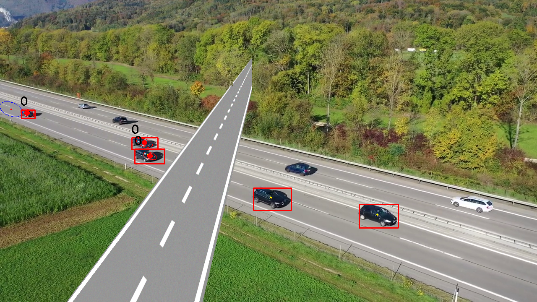
\includegraphics[width=\linewidth]{../../../experiments/\Ex/\Vs/YOLO/44}
        \caption{Frame number: 44.}
        \label{fig:\Ex-\Vs-\Set:01}
    \end{subfigure}
    \begin{subfigure}{0.48\textwidth}
        \centering
        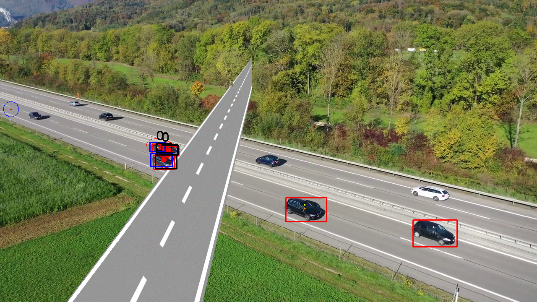
\includegraphics[width=\linewidth]{../../../experiments/\Ex/\Vs/YOLO/47}
        \caption{Frame number: 47.}
        \label{fig:\Ex-\Vs-\Set:02}
    \end{subfigure}
    \\
    \begin{subfigure}{0.48\textwidth}
        \centering
        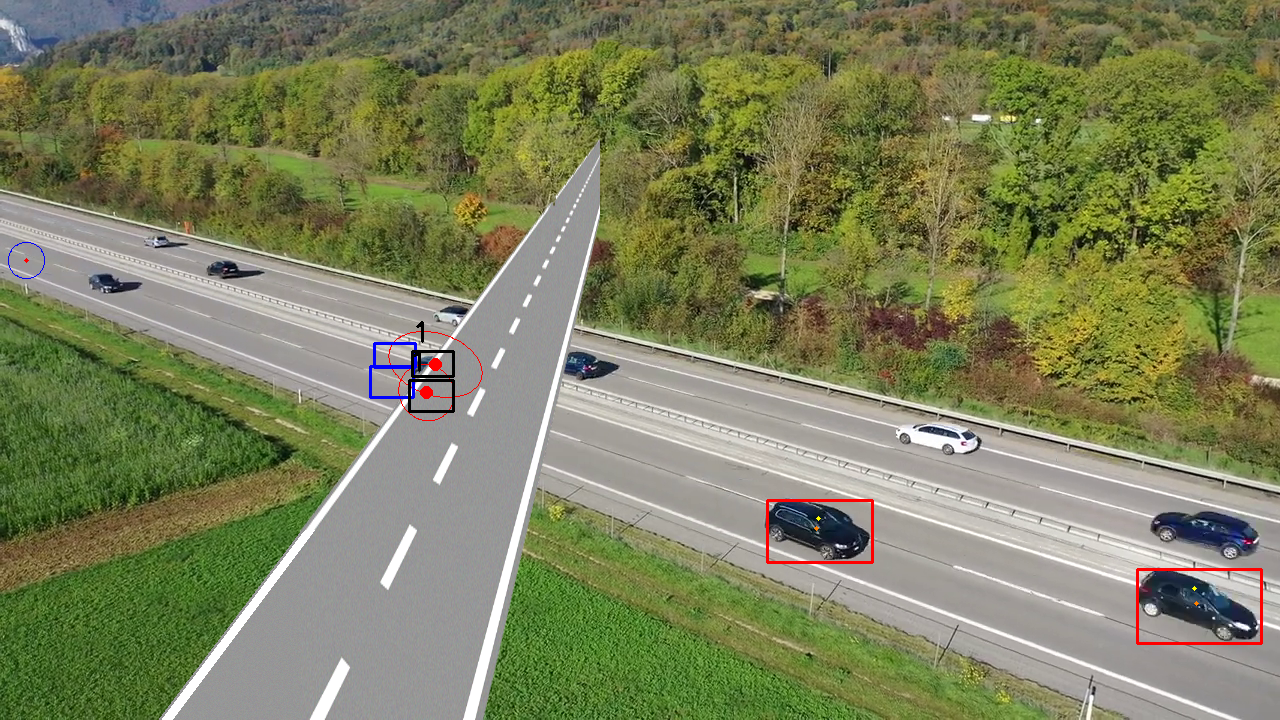
\includegraphics[width=\linewidth]{../../../experiments/\Ex/\Vs/YOLO/50}
        \caption{Frame number: 50.}
        \label{fig:\Ex-\Vs-\Set:03}
    \end{subfigure}
    \begin{subfigure}{0.48\textwidth}
        \centering
        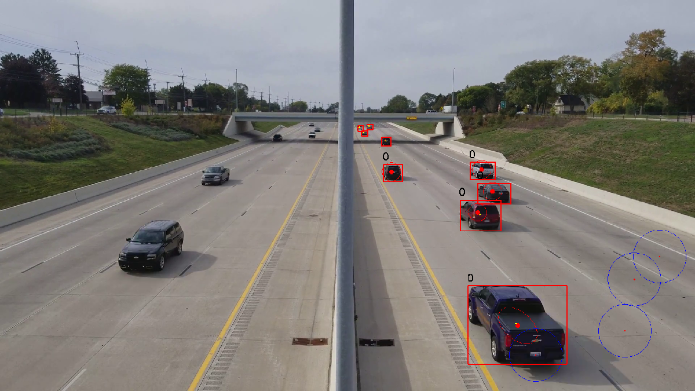
\includegraphics[width=\linewidth]{../../../experiments/\Ex/\Vs/YOLO/54}
        \caption{Frame number: 54.}
        \label{fig:\Ex-\Vs-\Set:04}
    \end{subfigure}
    \\
    \begin{subfigure}{0.48\textwidth}
        \centering
        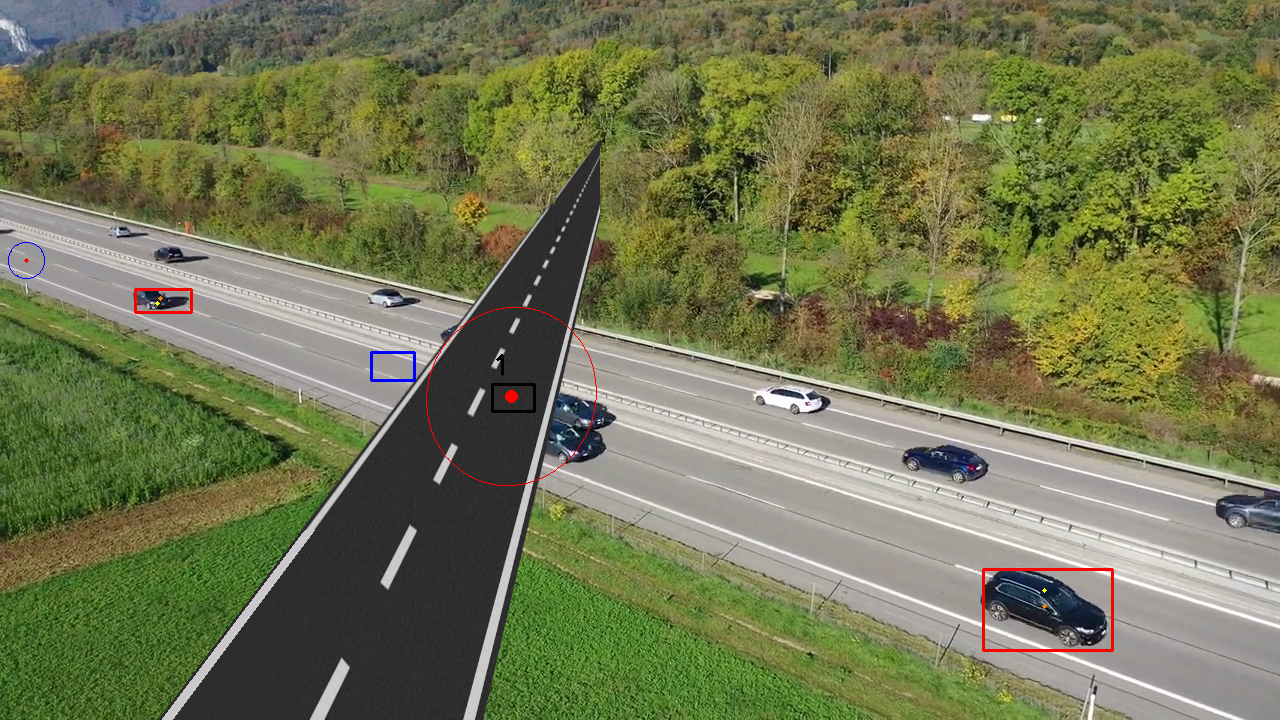
\includegraphics[width=\linewidth]{../../../experiments/\Ex/\Vs/YOLO/56}
        \caption{Frame number: 56.}
        \label{fig:\Ex-\Vs-\Set:05}
    \end{subfigure}
    \begin{subfigure}{0.48\textwidth}
        \centering
        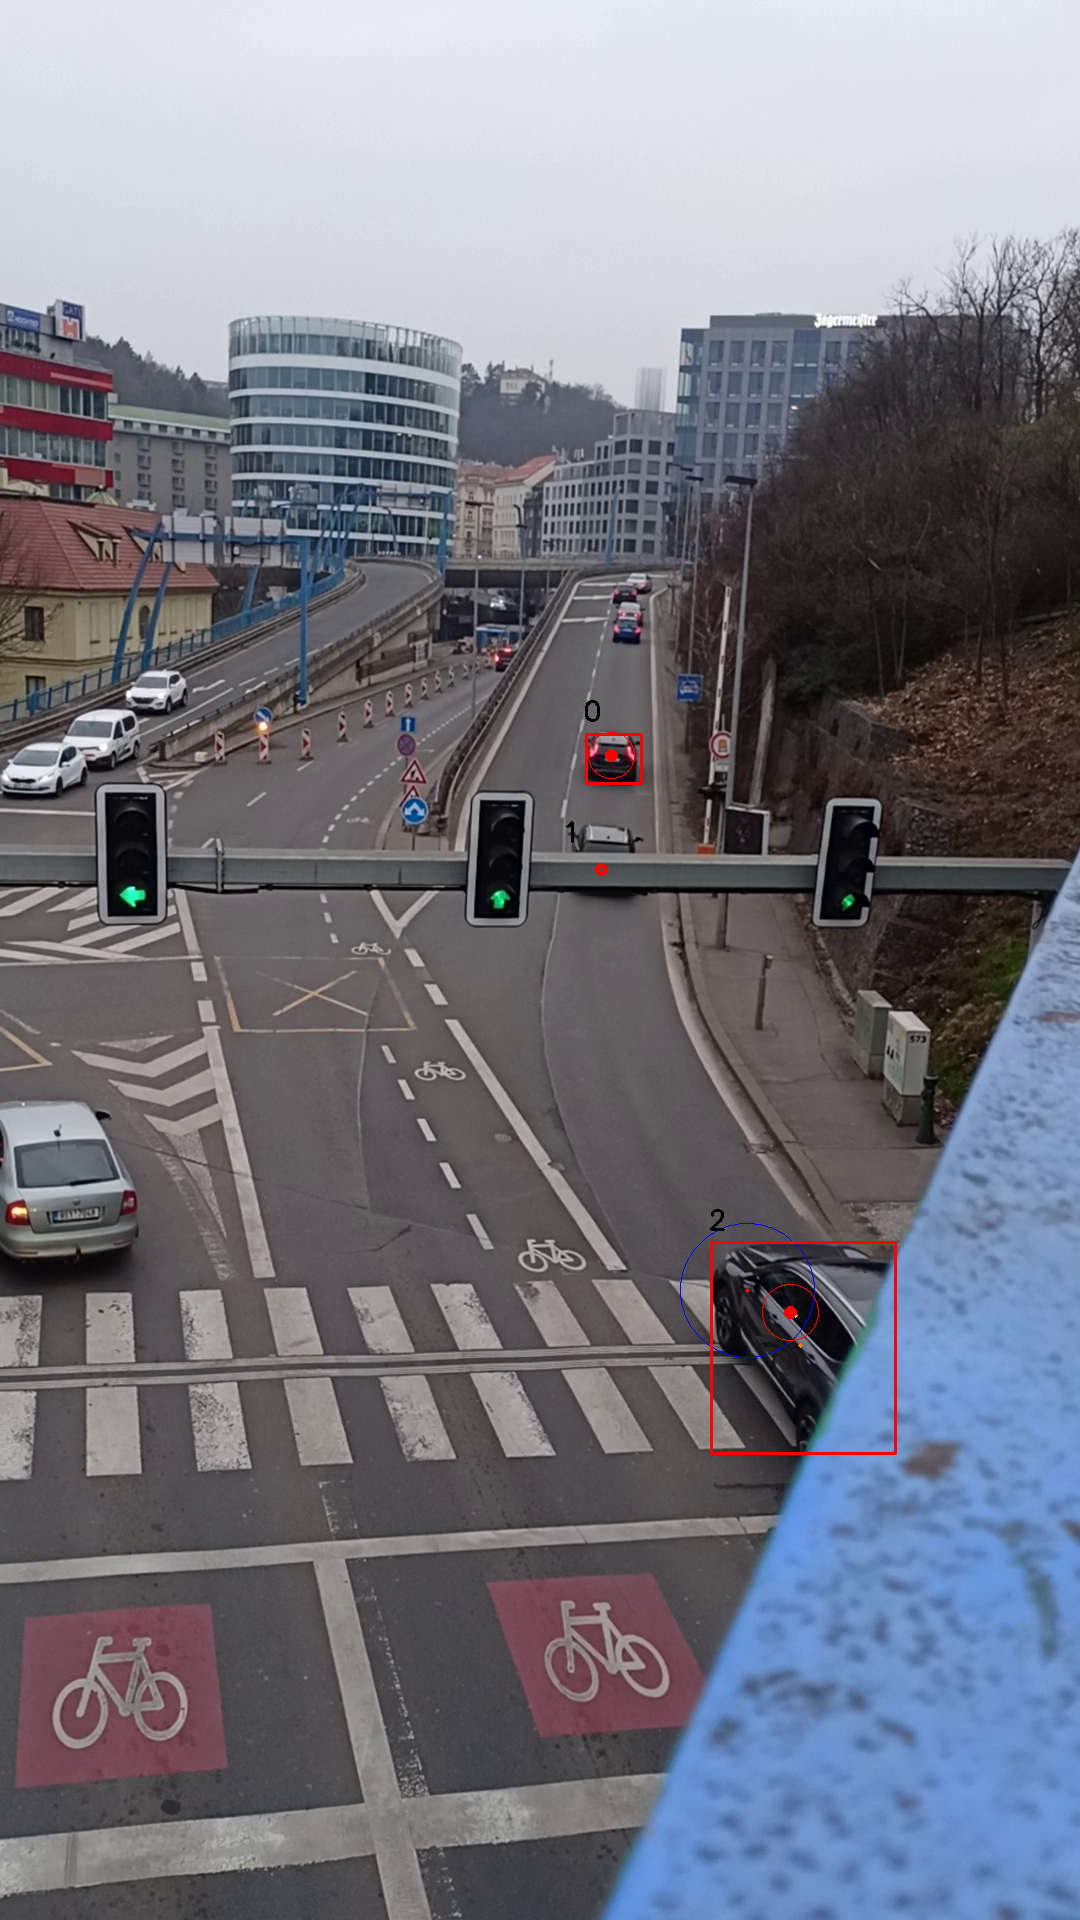
\includegraphics[width=\linewidth]{../../../experiments/\Ex/\Vs/YOLO/57}
        \caption{Frame number: 57.}
        \label{fig:\Ex-\Vs-\Set:06}
    \end{subfigure}
    \\
    \begin{subfigure}{0.48\textwidth}
        \centering
        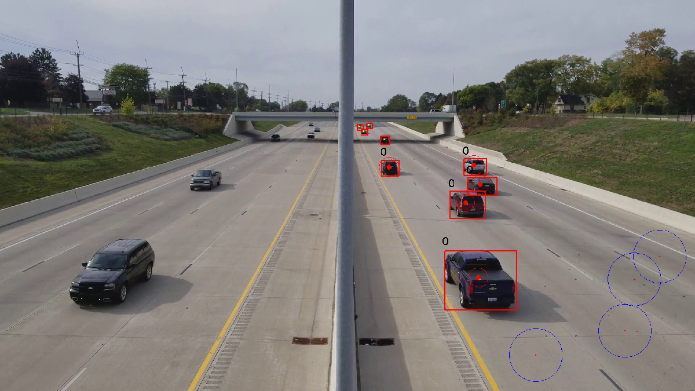
\includegraphics[width=\linewidth]{../../../experiments/\Ex/\Vs/YOLO/58}
        \caption{Frame number: 58.}
        \label{fig:\Ex-\Vs-\Set:07}
    \end{subfigure}
    \begin{subfigure}{0.48\textwidth}
        \centering
        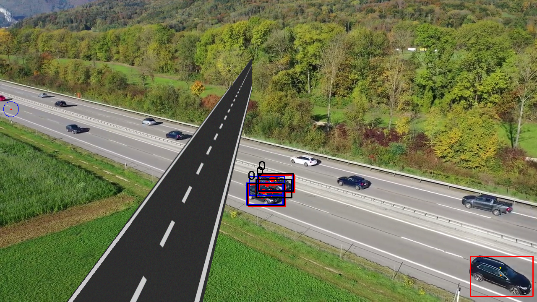
\includegraphics[width=\linewidth]{../../../experiments/\Ex/\Vs/YOLO/59}
        \caption{Frame number: 59.}
        \label{fig:\Ex-\Vs-\Set:08}
    \end{subfigure}
    \caption{Image sequence of tracked objects using the GM-PHD filter with the dynamic detection probability and YOLO only.}
    \label{fig:\Ex-\Vs-\Set}
\end{figure}

